\documentclass{article}
\usepackage{graphicx}
\usepackage{hyperref}
\usepackage{amsmath}
\usepackage[numbers,square]{natbib}
\usepackage{titlesec}
\titleformat{\section}{\normalfont\centering}{\thesection}{1em}{}

 \title{\textbf{CorcPUM: Efficient Processing Using Cross-Point Memory
 	via Cooperative Row-Column Access Pipelining and Adaptive
 	Timing Optimization in Subarrays}}
 \author{Paritosh Lahre \\ Indian Institute of Technology, Bhilai \\ 12341550 \\ paritoshl@iitbhilai.ac.in}
 \date{}
 \begin{document}
 	\maketitle
 	\textbf{Abstract—Emerging cross-point memory can in-situ perform
 		vector-matrix multiplication (VMM) for energy-efficient scientific
 		computation. However, parasitic-capacitance-induced row charg-
 		ing and discharging latency is a major performance bottleneck
 		of subarray VMM. We propose a memory-timing-compliant
 		bulk VMM processing-using-memory design with row access and
 		column access co-optimization from rethinking of read access
 		commands and µ-op timing. We propose row-level-parallelism-
 		adaptive timing termination mechanism to reduce tail latency of
 		tRCD and tRP by exploiting row nonlinear charging and bulk-
 		interleaved row-column-cooperative VMM access mechanism to
 		reduce tRAS and overlap CL without increasing column ADC
 		precision. Evaluations show that our design can achieve 5.03×
 		performance speedup compared with an aggressive baseline}
 	
 	\section*{I. INTRODUCTION}
 		Emerging cross-point memory can in-situ execute analog
 		vector-matrix multiplication (VMM) based on Ohm’s law and
 		Kirchhoff’s current law and is able to achieve energy-efficient
 		iterative solution of linear systems derived from complex prob-
 		lems in physics world, such as fluid dynamics, semiconductor
 		device simulation, circuit simulation, and structural mechan-
 		ics [1]–[4]. However, row charging and discharging latency
 		induced by both parasitic capacitance and line resistance is a
 		major performance bottleneck of high-frequency VMM oper-
 		ations performed on realistic-scale cell-arrays [5]. In reality,
 		due to the parasitic capacitance of wordlines and bitlines
 		and that of in between top and bottom electrodes of whole
 		row of cells, the internal cell-array core in cross-point RAM
 		operates in analog and has longer latency than the periphery
 		[6]–[8], to properly charge and discharge the RC parasitics and
 		guarantee the fundamental analog signal accuracy of wordlines
 		and bitlines in cell-arrays when executing VMM operations.
 		Previous works [1], [9] activated all the rows simultaneously
 		in a subarray during VMM execution and let all the columns
 		in a tile share one ADC. However, we observe that activating
 		all the rows simultaneously in a subarray is suboptimal for
 		performance improvement from the viewpoint of row access
 		and column access co-optimization. First, as more rows of
 		
 		\begin{figure}[h]
 			\centering
 			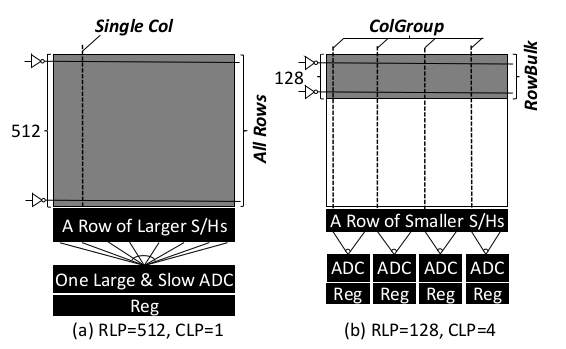
\includegraphics[width=0.7\linewidth]{images/fig1}
 			\caption{Tradeoff between Row-Level Parallelism and Col-Level Parallelism}
 			\label{fig:fig1}
 		\end{figure}

 		cells are activated or precharged simultaneously, these rows
 		have to be opened or closed more precisely to the target VP P
 		or ground potential in the time-varying charging or discharging
 		process, to guarantee the column ADC can correctly sense
 		the analog accumulated result. Due to the long tail latency of
 		row nonlinear charging, activating more rows simultaneously
 		significantly enlarges the required charging and discharging
 		latency. Second, activating more rows requires higher ADC
 		precision to sense the analog accumulated results at the end
 		of bitlines, and this will increase sense-amp-based ADC area,
 		latency and power [1], [10], [11]. As a result, more columns
 		have to share one ADC within a given subarray width, which
 		means that column-level parallelism (CLP) drops down when
 		row-level parallelism (RLP) increases, as shown in Fig. 1. Due
 		to decreased CLP, subarray row access has to wait for a longer
 		time before all the periphery column accesses traverse through
 		the ADC, wasting significant row access latency and cell-array
 		energy. Rather than activating all the rows simultaneously,
 		activating only a bulk of rows in parallel to reduce the row
 		activation and precharging latency, unlock the CLP, and reduce
 		the ADC sensing latency and row-buffer setup latency is able
 		to achieve performance improvement.
 		In this work, we identify new opportunities for optimizing
 		row charging and discharging latency of VMM accesses on
 		subarrays by co-optimizing row access and column access
 		and exploiting the µ-op interaction between subarray and
 		periphery. From rethinking of read access timing, we find that
 		VMM access needs a fine-grained landscape management of
 		polyphonic timing to fully exploit its massive parallelism. To
 		this end, we propose a memory-timing-compliant row-column-
 		
 		\begin{figure}[h]
 			\centering
 			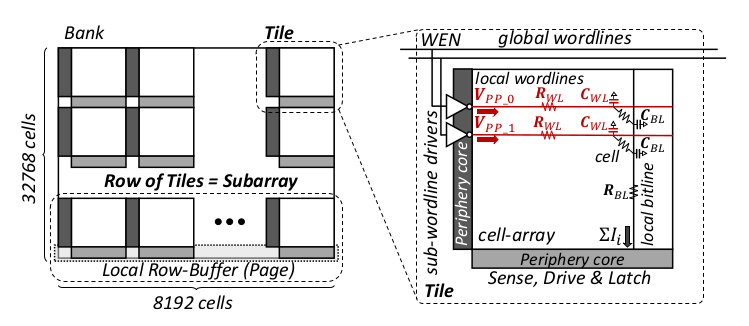
\includegraphics[width=0.7\linewidth]{images/fig2}
 			\caption{Cross-Point RAM Bank Organization (WEN: wordline enable signal)}
 			\label{fig:fig2}
 		\end{figure}
 		
 		cooperative processing-using-memory design with bulk VMM
 		access. We further propose fundamental mechanisms for re-
 		ducing internal core timing of bulk VMM operations on
 		subarrays: tRCD, tRP, tRAS, and CL. In summary, we make
 		the following contributions.
 		\begin{itemize}
 			\item We construct VMM as a memory column command and
 			propose a memory-timing-compliant bulk VMM access
 			mechanism from rethinking of µ-op of bank read access.
 			\item We propose a RLP-adaptive timing termination mecha-
 			nism exploiting row nonlinear charging to truncate the
 			unnecessary long tail latency of tRCD and tRP.
 			\item We further propose a bulk-interleaved coordinated VMM
 			operation mechanism to reduce tRAS and overlap CL
 			with row access and column access co-optimization.
 			\item We quantitatively evaluate our design with performance
 			improved by 5.03 times and energy reduced by 80.1\%.
 		\end{itemize}
 	
 	\section*{II. BACKGROUND AND MOTIVATION}
 		\begin{itemize}
 			\item[A.] \textit{Cross-Point RAM Bank Organization}
 				Cross-point oxide resistive RAM is divided into banks that
 				can be accessed in parallel with respect to each other [7], [12].
 				Fig. 2 presents the tall bank layout composed of a 2D array
 				of tiles. A tile comprises peripheral core transistors serving as
 				sense, drive, and latch functionalities and a cell-array where
 				each cell has a capacitor-like MIM lamellar structure with a
 				thin dielectric sandwiched between top and bottom electrodes,
 				using high-conductance state to store one and low-conductance
 				state to store zero. A row of tiles that share the same set of
 				global wordlines arranges in a subarray. Only one subarray can
 				be accessed in a bank at a time [12]. Here, a row refers to a row
 				of colinear cells, and a row of bitline latches is called a row-
 				buffer. The data stored in the local row-buffer in a subarray is
 				also called a page.
 			
 			\item [B.] \textit{Row Access and Column Access Commands}
 					We briefly review physical meanings of memory row access
 				and column access commands and timing parameters that
 				guarantee analog signal integrity without components conflict
 				[7], [13], as shown in Fig. 3.
 				\begin{enumerate}
 					\item Row ACTIVATE on Subarray (ACT): The ACT com-
 					mand accompanied by a row address first starts to open (pump)
 					a closed row to reach a stabilized activated state, and then
 					the row-buffer at the bitline periphery enables, to copy the
 					content of the whole row of cells into the row-buffer storage
 					nodes. The latency from the issue of ACT command to the
 					row-buffer stabilization is called the RAS n-to-CAS n Delay
 					
 					\begin{figure}
 						\centering
 						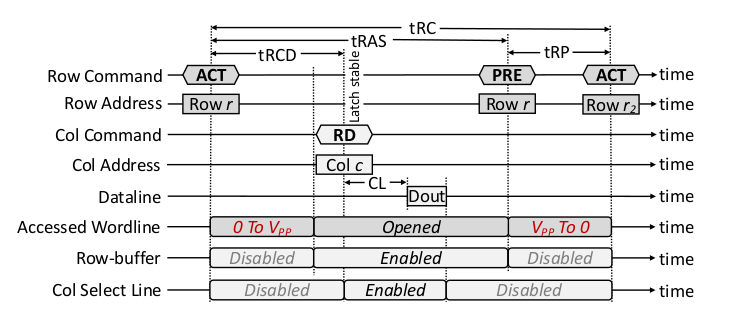
\includegraphics[width=0.7\linewidth]{images/fig3}
 						\caption{Internal Core Timing of Read Access on Cross-Point RAM Bank}
 						\label{fig:fig3}
 					\end{figure}
 					
 					time (tRCD), and the time interval when the row starts to open
 					until it is going to close is called the RAS n time (tRAS).
 					\item Row PRECHARGE on Subarray (PRE): The PRE com-
 					mand with a row address first immediately starts to close
 					the wordline already opened (VP P ) back to the completely
 					closed state and disables the row-buffer and precharges the
 					bitlines back to the baseline reference voltage for preparation
 					of accessing another row. The latency of this whole process
 					is called the RAS n Precharge time (tRP).
 					\item Column READ on Periphery (RD): When the row-buffer
 					storage nodes and bitlines are sufficiently stabilized during
 					activation, the RD command is issued with a column address
 					to enable a specific group of column select lines (CSL) and
 					transfer of a block of data from row-buffer storage nodes via
 					local datalines to destinated global I/O datalines. This whole
 					latency is called the read CAS n Latency (CL, a.k.a. tAA).
 				\end{enumerate}
 			
 			\item [C.] \textit{Rearchitecting Memory Access Commands for VMM}
 				From the above analysis, electrical read-out is sensing
 				at the end of the bitlines when the accessed row is fully
 				activated at the read voltage. Nondestructive VMM operation
 				is also sensing at the end of the bitlines with the exception
 				that multiple rows are activated simultaneously (wordlines
 				with zero-input are deactivated) and the data stored in the
 				subarray are already known. When we take binary voltage
 				(either VP P or ground) as wordline input and one-bit-per-
 				cell configuration, VMM operation is actually a native read
 				access except for multiple rows are activated. Motivated by the
 				similarities of read and VMM operations, we slightly modify
 				row ACT and PRE commands as follows and introduce VMM
 				as a column command to support bank VMM access.
 				\begin{enumerate}
 					\item Row ACT BULK on Subarray: ACT BULK is the same
 					as ACT except that multiple rows with non-zero input are
 					opened (pumped) to VP P . Here, a bulk of rows simultaneously
 					activated is called a RowBulk.
 					\item Row PRE BULK on Subarray: PRE BULK is the same
 					as PRE except that multiple rows at activated state are closed
 					(discharged) to ground potential.
 					\item Column VMM on Periphery: The column VMM com-
 					mand is analogous to column RD which fetches a part of
 					contents (determined by CLP) from row-buffer storage nodes
 					but goes through the data path for global shift-accumulation.
 				\end{enumerate}
 			
 		\end{itemize}
 			
 	\section*{III. CORCPUM DESIGN}
 		CorcPUM encompasses RLP-adaptive timing termination
 		and bulk-interleaved row-column-cooperative VMM access
 		mechanisms. The module hierarchy is shown in Fig. 4.
 		
 		\begin{figure}[h]
 			\centering
 			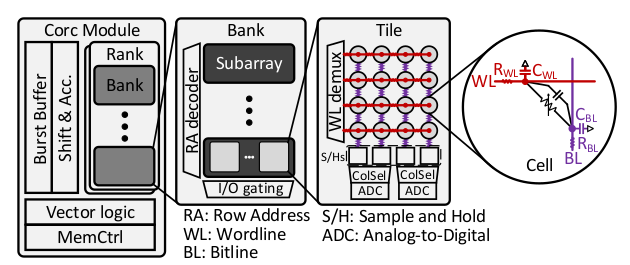
\includegraphics[width=0.7\linewidth]{images/fig4}
 			\caption{CorcPUM Module Hierarchy}
 			\label{fig:fig4}
 		\end{figure}
 		
 		\begin{figure}[h]
 			\centering
 			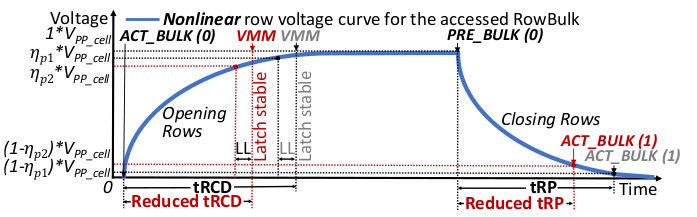
\includegraphics[width=0.7\linewidth]{images/fig5}
 			\caption{Physical Mechanism of RLP-Adaptive Timing Termination}
 			\label{fig:fig5}
 		\end{figure}
 		
 		\begin{itemize}
 			\item[A.] RLP-Adaptive Timing Termination Mechanism
 				The capacitor plate voltage never reaches full in RC circuits
 				unless the charging time is infinite. We first present first-order
 				analysis of the intrinsic relation between row charging coeffi-
 				cient and RLP. Fig. 5 captures the row voltage curve during
 				row activation and precharging phases of subarray VMM. We
 				observe that row charging and discharging processes are highly
 				nonlinear and asymptotic to VP P and ground potential, and
 				both tRCD and tRP have a very long tail latency to guarantee
 				proper charging and discharging. We find that if more rows
 				are activated simultaneously in a subarray, these rows have
 				to reach more close to VP P and ground states, therefore
 				having a longer tail latency of tRCD and tRP. If we view
 				the cell I-V curve as linear at small voltages, when all the
 				RowBulk-corresponded wordlines are input high and all the
 				cells on the bitline segment inside the RowBulk are at the high-
 				conductance state, the maximum accumulative relative error at
 				the end of the bitline can be expressed as $RE_{Acc} = RLP * (1 - \eta_{\rho})$, where $0 < \eta_{\rho} < 1$ is the row charging coefficient.
 				REAcc should not exceed the ADC sensing static noise margin
 				$RE_{margin} = 1/(2*(2^{ADC{\_}{bits}} - 1))$. We invert the contents
 				of a column if it contains all ‘1’s, therefore ${ADC}\_{bits} = \log_2 (RLP)$, when \textit{RLP} $\geq$ 2 [1]. We can derive the lower
 				boundary of $\eta_{\rho}$ as ${\eta_{\rho}}^{LB} = 1 - 1/(2*{RLP}*({RLP} - 1))$. We can
 				see that ${\eta_{\rho}}^{LB}$ monotonically increases with RLP increasing. To
 				reduce row access latency, we propose a RLP-adaptive timing
 				termination (RATT) mechanism to truncate the unnecessary
 				long tail latency of tRCD and tRP during row activation and
 				precharging by exploiting row nonlinear charging dynamics
 				in light of RLP. Table I shows RLP-dependent row charging
 				coefficient and correlated latency profile to the extreme extent
 				in 512×256 cell-arrays with sub-wordline drivers placed in
 				the middle [1] obtained via HSPICE simulation. Activating
 				all 512 rows will even take 34.7 ns tRCD and 24.8 ns tRP. By
 				reducing RLP, tRCD and tRP can be reduced.
 			\item[B.] \textit{Bulk-Interleaved Row-Column-Cooperative VMM Access}
 				We further co-optimize row access and column access to
 				reduce the row activation time (tRAS) of VMM and improve
 				hardware spatiotemporal utilization from three aspects. The
 				overall stripy operation mechanism is shown in Fig. 6.
 				
 				\begin{figure}[h]
 					\centering
 					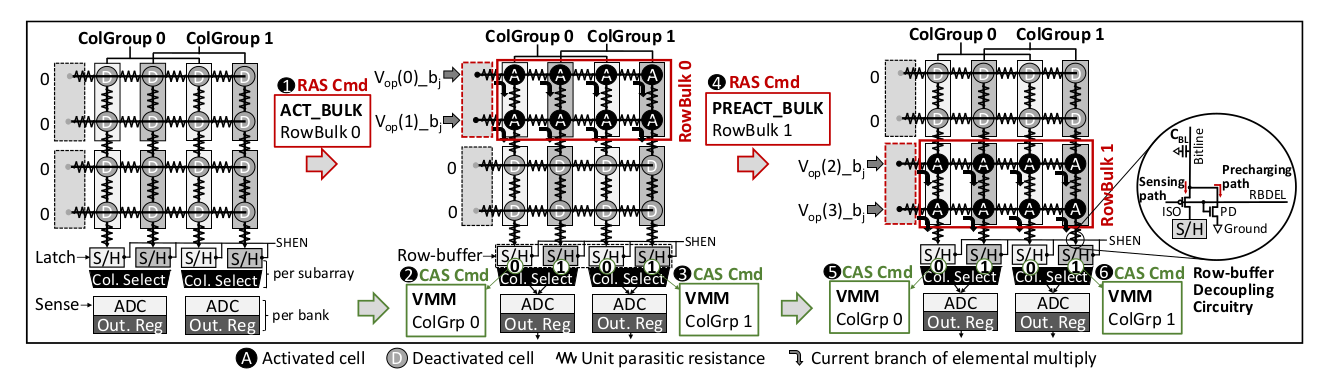
\includegraphics[width=0.7\linewidth]{images/fig6}
 					\caption{Memory-Native Subarray VMM Access Operation Mechanism (RBDEL: row-buffer decouple line, PD: pull down, SHEN: S/H enable)}
 					\label{fig:fig6}
 				\end{figure}
 				
 				\begin{center}
 					TABLE I \\
 					RLP IMPACT ON ROW CHARGING COEFFICIENT AND MIN. LATENCY
 					\begin{tabular}{|c|c|c|c|c|c|c|c|} \hline
 						RLP & 4 & 8 & 16 & 32 & 64 & 128 & 256 \\ \hline
 						${\eta_{\rho}}^{\textit{LB}} (\%)$ & 95.83 & 99.11 & 99.79 & 99.95 & 99.988 & 99.997 & 99.999 \\ \hline
 						tRCD (ns) & 8.6 & 13 & 17.1 & 21.1 & 25.1 & 28.7 & 31.2 \\ \hline
 						tRP (ns) & 6.4 & 9.7 & 12.7 & 15.6 & 18.5 & 21.0 & 22.4 \\ \hline
 					\end{tabular}
 				\end{center}	
 		\end{itemize}
 		
 		\begin{enumerate}
 			\item[1)] \textit{Parallelizing Precharging with Row-Buffering via Cir-
 				cuitry Decoupling:} The precharge phase involves both word-
 			line closing and bitline precharging. For cross-point RAM, we
 			can precharge the bitlines to ground when the wordlines are
 			not completely closed because bitline precharging does not
 			disturb the cells being closed. However, the row-buffer and
 			bitline precharge circuitry are exclusive and cannot be enabled
 			simultaneously due to the circuit connection property [6], [14],
 			and a conflict between bitline precharging and row-buffering
 			exists. In cross-point RAM, closing the wordline immedi-
 			ately changes the bitline current, thus the row-buffer storage
 			nodes must be decoupled from the bitlines at the onset of
 			precharging. We want to hold all the bitlines to ground during
 			wordlines closing and meanwhile decoupling the bitlines from
 			row-buffer to let the row-buffer still be kept enabled and holds
 			its content without disturbed by the change of bitline currents.
 			To this end, we propose parallelizing precharging with row
 			buffering (PPRB) via a decoupling circuitry which consists of
 			a NMOS pull-down transistor and a PMOS isolation transistor
 			to separate the precharging and the sensing paths, as shown in
 			the right side of Fig. 6. By enabling the row-buffer decouple
 			line (RBDEL), the bitline is decoupled from the row-buffer
 			and precharged to ground. When the row-buffer is enabled,
 			disabling the RBDEL to connect the bitline to the row-buffer.
 			Since the charges stored in the parasitic capacitance makes
 			the bitline have inertia and be able to keep its state, we can
 			properly switch the bitline from connecting to the precharging
 			path to connecting to the sensing path by enabling the RBDEL.
 			With circuitry decoupling, precharging and row-buffering can
 			be parallelized to reduce tRAS, as shown in Fig. 7(b).
 			
 			\item[2)] \textit{RowBulk Interleaving by Exploiting Axisymmetry of Row
 				Charging and Discharging:} Due to the nondestructive nature
 			of VMM operation, tRAS is dependent since the cell content
 			restoration process is no longer required. However, rows
 			opening and closing processes are still dominant in raw VMM
 			access latency shown in Fig. 7(a). Based on the observation
 			that row charging and discharging processes are axisymmetric,
 			we further propose a RowBulk interleaving (RBI) mechanism
 			with a ACT-when-PRE feature to overlap row activation and
 			precharging latency in the raw VMM access process. The
 			current RowBulk is precharged to $(1 - \eta_{\rho}) * V_{PP}$ when the
 			next RowBulk is activated to $\eta_{\rho} * V_{PP}$ , where $\eta_{\rho}$ is the row
 			charging coefficient. Based on the axisymmetry, we can derive
 			$tRCD = tRP + LL$, where $LL = k_{LL} \log_2 RLP$ is the
 			row-buffer latching latency, and $k_{LL}$ is the latency slope [6].
 			RBI mechanism guarantees that the current RowBulk is fully
 			discharged when the next RowBulk is fully opened. Exactly
 			when the current RowBulk completes its precharging process,
 			the row-buffer can be re-enabled to start re-latching new data
 			for the next RowBulk. RBI requires modification to the local
 			
 			\begin{figure}[h]
 				\centering
 				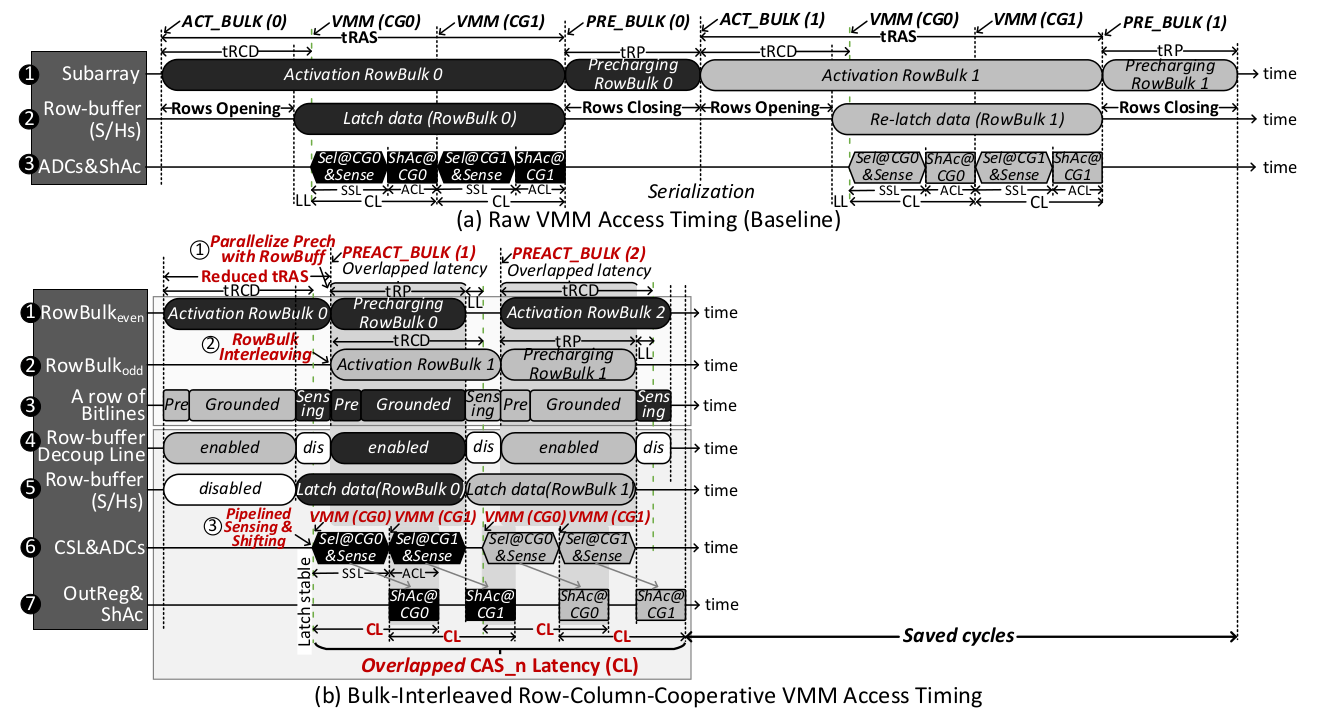
\includegraphics[width=0.7\linewidth]{images/fig7}
 				\caption{Reducing tRAS and Overlapping CL via Memory-Timing-Compliant Bulk-Interleaving and Coordinated Row-Column Access Pipelining}
 				\label{fig:fig7}
 			\end{figure}
 			
 			row address decoder and needs twice number of sub-wordline
 			drivers to simultaneously select two adjacent RowBulks for
 			precharging and activation respectively.
 			We introduce the PREACT\_BULK command as an ad-
 			vanced alternative to the PRE\_BULK command to enable the
 			RBI mechanism that issues the precharge with auto-activate
 			of the next RowBulk. One important benefit of RBI is that
 			it does not increase the required column ADC precision,
 			because the number of activated rows does not change at the
 			time the row-buffer is enabled. Note that there is a timing
 			constraint that we cannot issue the activate command of the
 			current RowBulk before issuing the precharge command of the
 			previous RowBulk because the bitline S/Hs have to wait until
 			the precharging process of the previous RowBulk completes.
 			
 			\item[3)] \textit{Overlapping CL via Pipelining Sensing and Shifting:} In
 			the raw VMM access timing shown in Fig. 7(a), the periphery
 			column-access CL latency comprises the ADC sensing latency
 			(SSL) together with the shift-accumulate latency (ACL), where
 			SSL = kSSL log2 (RLP ) [10]. We further propose pipelining
 			sensing and shifting (PSS) between bank ADC sensing and
 			global shift-accumulate logic to overlap the CL latency and
 			reduce the latency between adjacent VMM commands by
 			adding an output register whose bit width is no less than the ADC precision at the end of each ADC. Output registers across
 			all banks can be viewed as a global row-buffer. Therefore, the
 			issue of the next VMM command does not have to wait for
 			the shift-accumulate step of the current VMM to complete.
 			In this manner, tRAS is reduced, as shown in Fig. 7(b). We
 			can further derive $tRAS = (\eta_{cols}/\eta_{rows}) * RLP * k_{SSL} * \log_2(RLP) + k_{LL}*\log_2RLP$ , where $\eta_{rows}$ and $\eta_{cols}$ are the
 			number of rows and columns in a subarray respectively. Since
 			the accessed row address has high locality, we use the open-
 			page row-buffer-management policy for VMM accesses, which
 			only issues subsequent column commands in a burst mode
 			without repeatly issuing the same row access command when
 			the row-buffer hits, which saves row cycles. Fig. 8 shows the
 			polyphonic memory timing diagram with overlapped pattern
 			of row access and column access.
 		\end{enumerate}
 	
 	\section*{IV. EVALUATION}
 		\begin{itemize}
 			\item[A.] \textit{Experimental Setup} \\
 			To determine the latency and power of time-varying row
 			charging and discharging processes in cross-point RAM, we
 			write a C-coded script to generate the full HSPICE circuit
 			netlist of HfO$_x$ -based cell-array [15]. The array-level parasitic
 			resistance and capacitance are extracted from [7], [16]. We
 			
 			\begin{figure}[h]
 				\centering
 				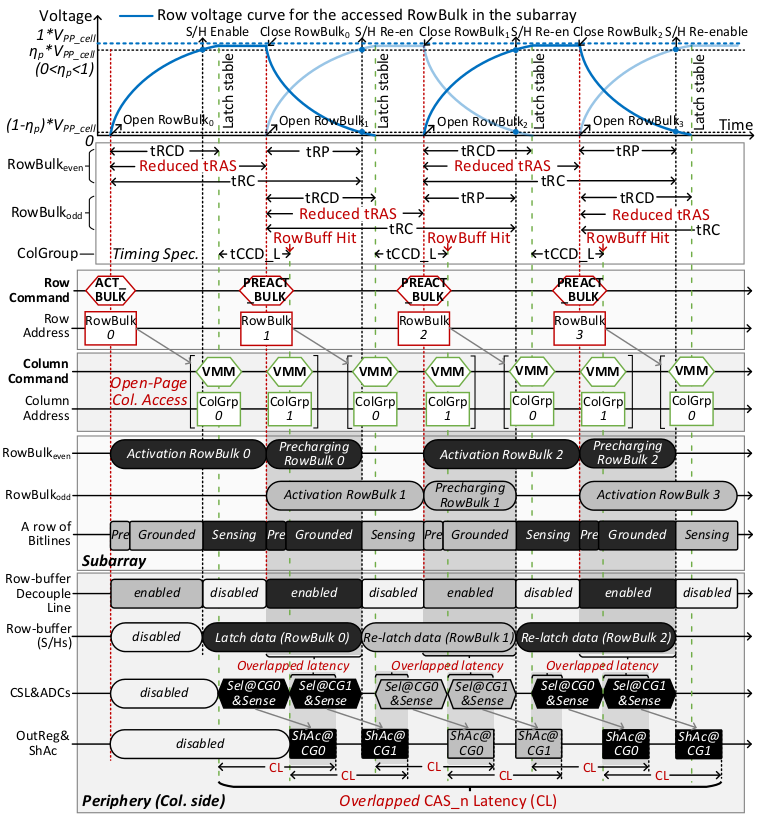
\includegraphics[width=0.7\linewidth]{images/fig8}
 				\caption{Polyphonic Timing of Bulk-Interleaved Cooperative Row-Col. Access}
 				\label{fig:fig8}
 			\end{figure}
 			
 			\begin{table}[h]
 				\centering
 				TABLE 2 \\ HARDWARE CONFIGURATION
 				\begin{tabular}{|p{13cm}|}
 					\hline
 					Dual ranks, 64 banks/rank, bank size 32768×8192, 64 subarrays/bank, tile size 512×256 with sub-wordline drivers placed in the middle, HfOx MIM cell, global shift-accumulate and vector logic parallelism 1024, $G_\text{on} = 1 \times 10^{-6} \, \text{S}$, $G_\text{off} = 1 \times 10^{-8} \, \text{S}$, one-bit-per-cell, binary voltage input, feature size 14 nm, Tungsten $R_l = 14.3 \, \Omega$, $C_l = 0.4883$ fF, CMIM = 3.0 fF, $V_{\text{PPVMM}} = 1.0$ V, $t_{RCD}$ and $t_{RP}$ are shown in Table I, $k_{LL} = 1.1$, $k_{SSL} = 0.25$, ACL = 0.2, RLP = 16, cell-array VMM power: 3 mW. \\ 
 					\hline
 				\end{tabular}
 			\end{table}
 			model the CMOS peripheral components of cross-point mem-
 			ory subarray including decoders and select logic in CACTI.
 			We follow [17] to scale the ADC power consumption for
 			different ADC resolution. We simulate 10 MB eDRAM burst
 			buffer using CACTI with 14 nm parameters from [18]. The
 			global shift-accumulate component, vector logic and control
 			are implemented in Synopsys Design Compiler using TSMC
 			130 nm cell library and scaled to 14 nm technology size to
 			determine latency, power and area of global periphery. The
 			memory parameters are listed in Table II. To reduce bitline
 			sensing precision requirement during VMM, we only store
 			one bit in each cell. We evaluate the proposed design by
 			SuiteSparse matrix collection [4] benchmarks and restructure
 			the biconjugate gradient stabilized (BICGSTAB) method [19]
 			in MATLAB for computation in cell-arrays with maximum
 			iterations of 15000 for solving linear systems. We implement
 			double-precision floating-point representation as [1] and store
 			non-zero matrix blocks in bit-sliced manner. We set the EnSC
 			[1] as the baseline to compare with our proposal.
 			\item[B.] \textit{Result} \\
 				\begin{enumerate}
 					\item \textit{Performance:} Fig. 9 shows that CorcPUM achieves an
 					average overall speedup of 5.03 times compared with the
 					EnSC baseline across the benchmarks. Although other vector 
 					
 					\begin{figure}[h]
 						\centering
 						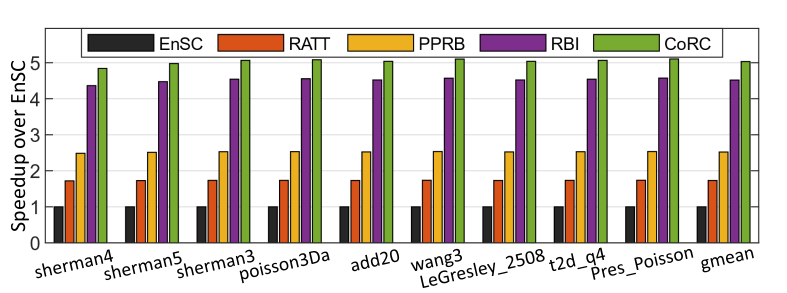
\includegraphics[width=0.7\linewidth]{images/fig9}
 						\caption{Speedup of CorcPUM over the EnSC Baseline}
 						\label{fig:fig9}
 					\end{figure}
 					
 					\begin{figure}[h]
 						\centering
 						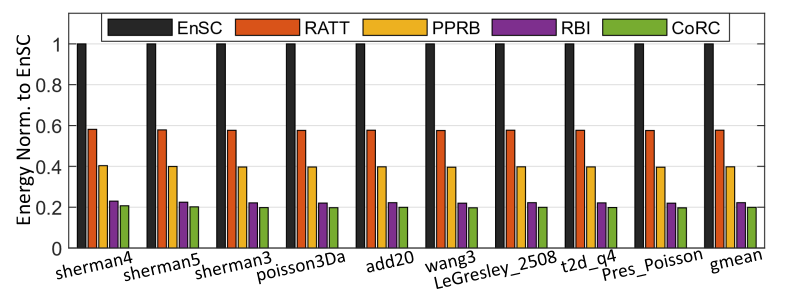
\includegraphics[width=0.7\linewidth]{images/fig10}
 						\caption{Energy Consumption of CorcPUM Normalized to the EnSC Baseline}
 						\label{fig:fig10}
 					\end{figure}
 					
 					\begin{figure}[h!]
 						\centering
 						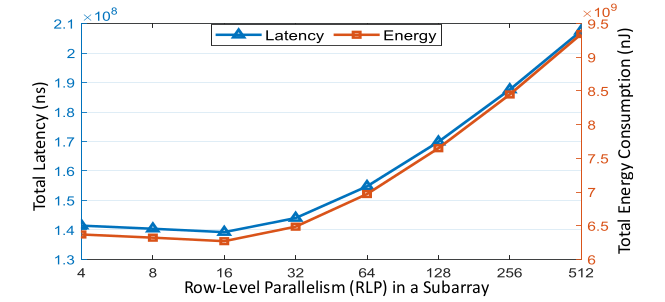
\includegraphics[width=0.7\linewidth]{images/fig11}
 						\caption{Sensitivity of Overall Latency and Energy to RLP}
 						\label{fig:fig11}
 					\end{figure}

 					
 					operations in BICGSTAB algorithm with O($n$) complexity
 					implemented by CMOS periphery cannot be directly sped
 					up, CorcPUM has a significant performance enhancement
 					normalized to the baseline, because each BICGSTAB iteration
 					contains two VMM operations with O($n^2$) complexity which
 					is dominant in solving linear systems and we proportionally
 					optimize row and column accesses and leverage bank paral-
 					lelism to in-situ perform VMM in cross-point RAM.
 					
 					\item \textit{Energy:} The energy consumption results breakdown of
 					CorcPUM is shown in Fig. 10. The overall energy is reduced
 					by 80.1\% on average compared with the baseline, due to
 					the superior latency reduction without significantly increasing
 					the power consumption. Compared with the baseline, RATT,
 					PPRB, RBI, and PSS components cumulatively increase the
 					total power consumption by 0.002\%, 0.343\%, 0.344\%, 0.346\%
 					across the benchmarks on average respectively.
 					
 					\item \textit{Sensitivity to RLP:} RLP is an important role that affects
 					the performance in CorcPUM design. Fig. 11 shows the
 					sensitivity of total latency and energy on average across the
 					benchmarks to RLP. We can see that keeping RLP at a
 					relatively low value can reduce latency. However, row-buffer
 					latching total latency increases if RLP drops too low. Due to
 					the competitive effect between row latching times and column
 					sensing times induced by the tradeoff between RLP and CLP,
 					taking a medium RLP achieves optimal performance.
 					
 					\item \textit{Hardware Overhead:} In CorcPUM design, RATT re-
 					quires a global lookup table to store RLP-adaptive tRCD and
 					tRP timing parameters, as shown in Table I. These values are
 					stored in the reserved zone of the extreme memory profile of extended serial presence detect. PPRB requires additional
 					two transistors per bitline and a row-buffer decouple line
 					per bank, and these incur 0.3\% area overhead. RBI requires
 					modification to the local row address decoder to select the next
 					adjacent RowBulk for activation while the current RowBulk
 					for precharging. This modification enlarges the area of local
 					row decoders by 6\% and needs twice number of sub-wordline
 					drivers per bank. PSS requires a register whose width equals
 					to the ADC precision at the end of each ADC per bank.
 					Compared with the baseline, these together increases the area
 					by 0.3\% and incurs 32 KB storage overhead.
 				\end{enumerate}
 		\end{itemize}
	\section*{V. RELATED WORK}
		\textit{Processing using Cross-Point RAM for Scientific Comput-
		ing.} Feinberg et al. [1] proposed a processing-using-memory
		design with a floating-point representation and matrix block
		placement. Feinberg et al. [2] studied the role of ADC preci-
		sion on subarray result accuracy of in-situ VMM operations.
		Le Gallo et al. [3] proposed an in-situ linear system iterative
		solver using phase-change memory. Zidan et al. [20] proposed
		a bit-sliced precision extension technique for in-situ VMM
		operations. Sun et al. [21] proposed a feedback-based linear
		system solver leveraging cross-point arrays. These works
		mainly explored operand representation and mapping on cross-
		point arrays. The intrinsic latency problem of data-intensive
		VMM on cross-point cell-arrays is yet to be solved.
		
		\textit{Architecting Low-Latency Memory Operation Timing.} Kim
		et al. [12] added another group of local datalines to overlap
		activating with write recovery and precharging in DRAM
		banks. Lee et al. [22] added isolation transistors into bitlines to
		physically separate the subarray to reduce the latency induced
		by bitline capacitance. Seongil et al. [14] proposed to add
		isolation transistors between the exclusive bitline equalizer and
		sense amplifier to overlap precharging with row-buffering for
		reducing latency. Lung et al. [23] constructed bank-interleaved
		memory access timing for reducing latency of cross-point
		RAM. Kim et al. [7] studied RC parasitics-induced latency
		and optimized read access timing via bitline segmentation.
		Oh et al. [24] constructed pipelined read access timing for
		resistance-based memory with page-mode column accesses.
		
		\textit{Exploiting Row Nonlinear Charging for Reducing Latency.}
		Zhang et al. [25] proposed a restoration truncation mechanism
		during row activation period without significantly sacrificing
		data-retention time and bitline sensing resolution for DRAM
		access. Wang et al. [26] proposed a charge-level-adaptive
		bitline partial restoration mechanism to reduce long tail latency
		of row activation period in DRAM access. To the best of our
		knowledge, this is the first work that enables memory-timing-
		compliant bulk VMM operation functionality on cross-point
		RAM with row access and column access co-optimization.
 		
	\section*{VI. CONCLUSION}
		Parasitic capacitance is a fundamental physics property that
		circumscribes the latency of high-frequency analog VMM
		operations on cross-point RAM cell-arrays. We presented
		physical insights into parasitic RC effects on VMM latency and analyzed the polyphonic memory timing of subarray
		VMM access. We proposed RLP-actuated timing termination
		mechanism and bulk-interleaved VMM operation mechanism
		with row access and column access co-optimization to reduce
		cross-point RAM internal core latency with negligible power
		overhead. The proposed processing-using-memory design can
		enable memory-timing-compliant bulk VMM processing in a
		memory-centric fashion for efficient hardware execution of
		data-intensive scientific computation.
	
	\bibliographystyle{plainnat}
	\bibliography{references}
 \end{document}